\chapter{Experimental Approach and Procedure towards Optical Pumping} 
This section explains the setup and approach toward realizing optical pumping on the NASABEC machine. The main apparatus is ColdQuanta's RuBECi 2D+ and 3D MOT Chamber system. This section does not discuss the equipment setup for the 2D and 3D magneto-optical trap, repump beam, transfer coils, or ColdQuanta's Quadrupole Coil Assembly. More information on this equipment and the laser cooling steps can be found in previous alumni theses\cite{sshea}\cite{mcwik}\cite{dpaseltiner}.
\newline

\section{Building an Optical Pathway to the NASABEC}
The first step in creating an optical pumping process is getting light to the RuBECi apparatus. The table that houses the laser and laser amplifier is about 1.5 meters away from the table where the RuBECi machine is mounted. In addition, there was no laser power designated for optical pumping. The setup for this section is shown in \textbf{Figure 3.1} and \textbf{Figure 3.2}. 

\begin{figure}[h!]
\begin{center}
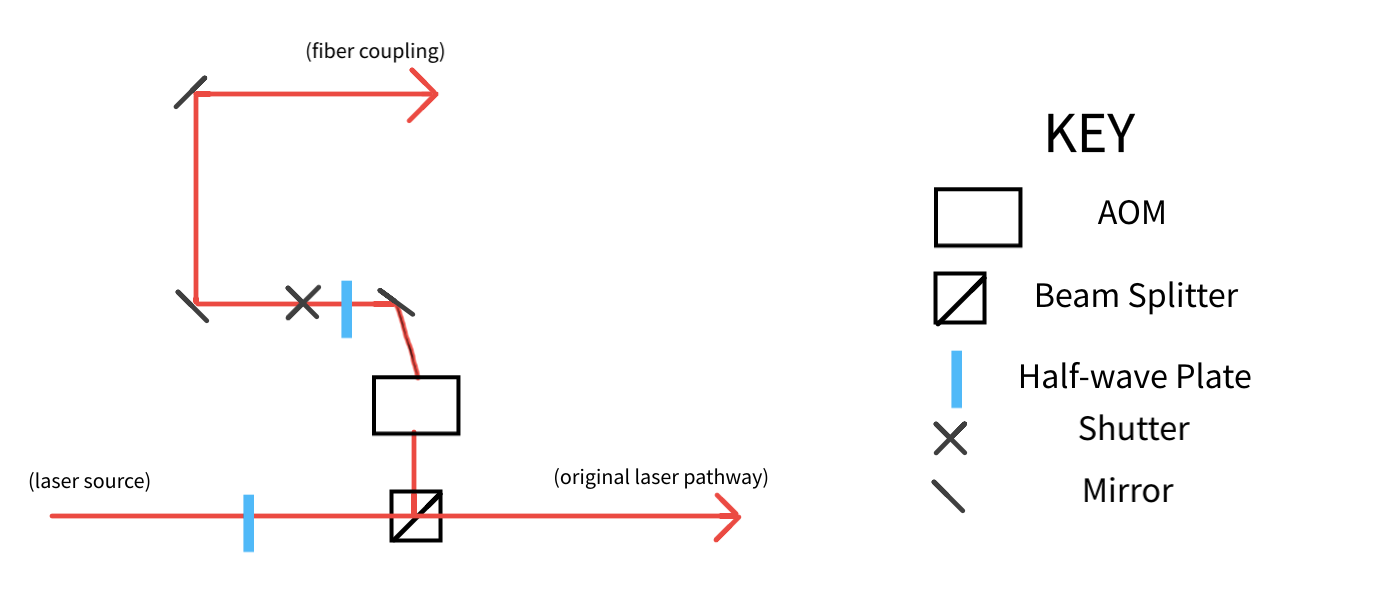
\epsfig{file=fig_setup_drawing.png, scale = .6}
\end{center}
\caption{A schematic diagram of the optical pathway for to get light to the RuBECi machine. }
\end{figure}

\begin{figure}[h!]
\begin{center}
\epsfig{file=fig_first_table.jpg, scale = .1195}
\end{center}
\caption{A picture of the optical pathway for to get light to the RuBECi machine. }
\end{figure}

To create this optical pathway, some of the laser's power was extracted with a half-wave plate and beam splitter. These devices were placed in the laser's path. Then the half-wave plate was rotated so that so about $8mW$ of power was reflected by the beam splitter to be used for optical pumping. 

At that point, an acousto-optic modulator and mechanical shutter are used to control when light is coupled in the optical fiber. The acousto-optic modulator responds fast to electrical signals and changes the laser pathway so that the optical pumping process only happens when required\cite{aom}. The mechanical shutter responds slower, but is used to completely block all light to ensure there is no small amount of light being coupled into the optical fiber\cite{fiberoptics}.

From there, a half-wave plate, two mirrors, an A375TM lens, and an adjustable cage mount are used to couple light into an optical fiber which can carry light to the RuBECi machine. This coupling process is tricky. The optical fiber only takes the Gaussian mode of the incoming light into a very small aperture. The result is searching for a maximum efficiency in a 5D space: two dimensions for the lasers (closest) position relative to the center of the aperture, two dimensions for the laser's angle at the aperture, and one dimension is the lens distance, or the laser's diameter, at the aperture of the optical fiber. 

 Optical fiber coupling efficiencies typically range from $45\%$ to $65\%$. The light in this setup was coupled with an efficiency of $65\%$. The 10 meter optical fiber was then ziptied to other optical fibers brought to the NASABEC machine and then mounted near one of the quadrupole coil set's principle axes for reasons described in \textbf{Chapter 1.2.3}. The mount is shown in \textbf{Figure 3.3}.

 \begin{figure}[h!]
\begin{center}
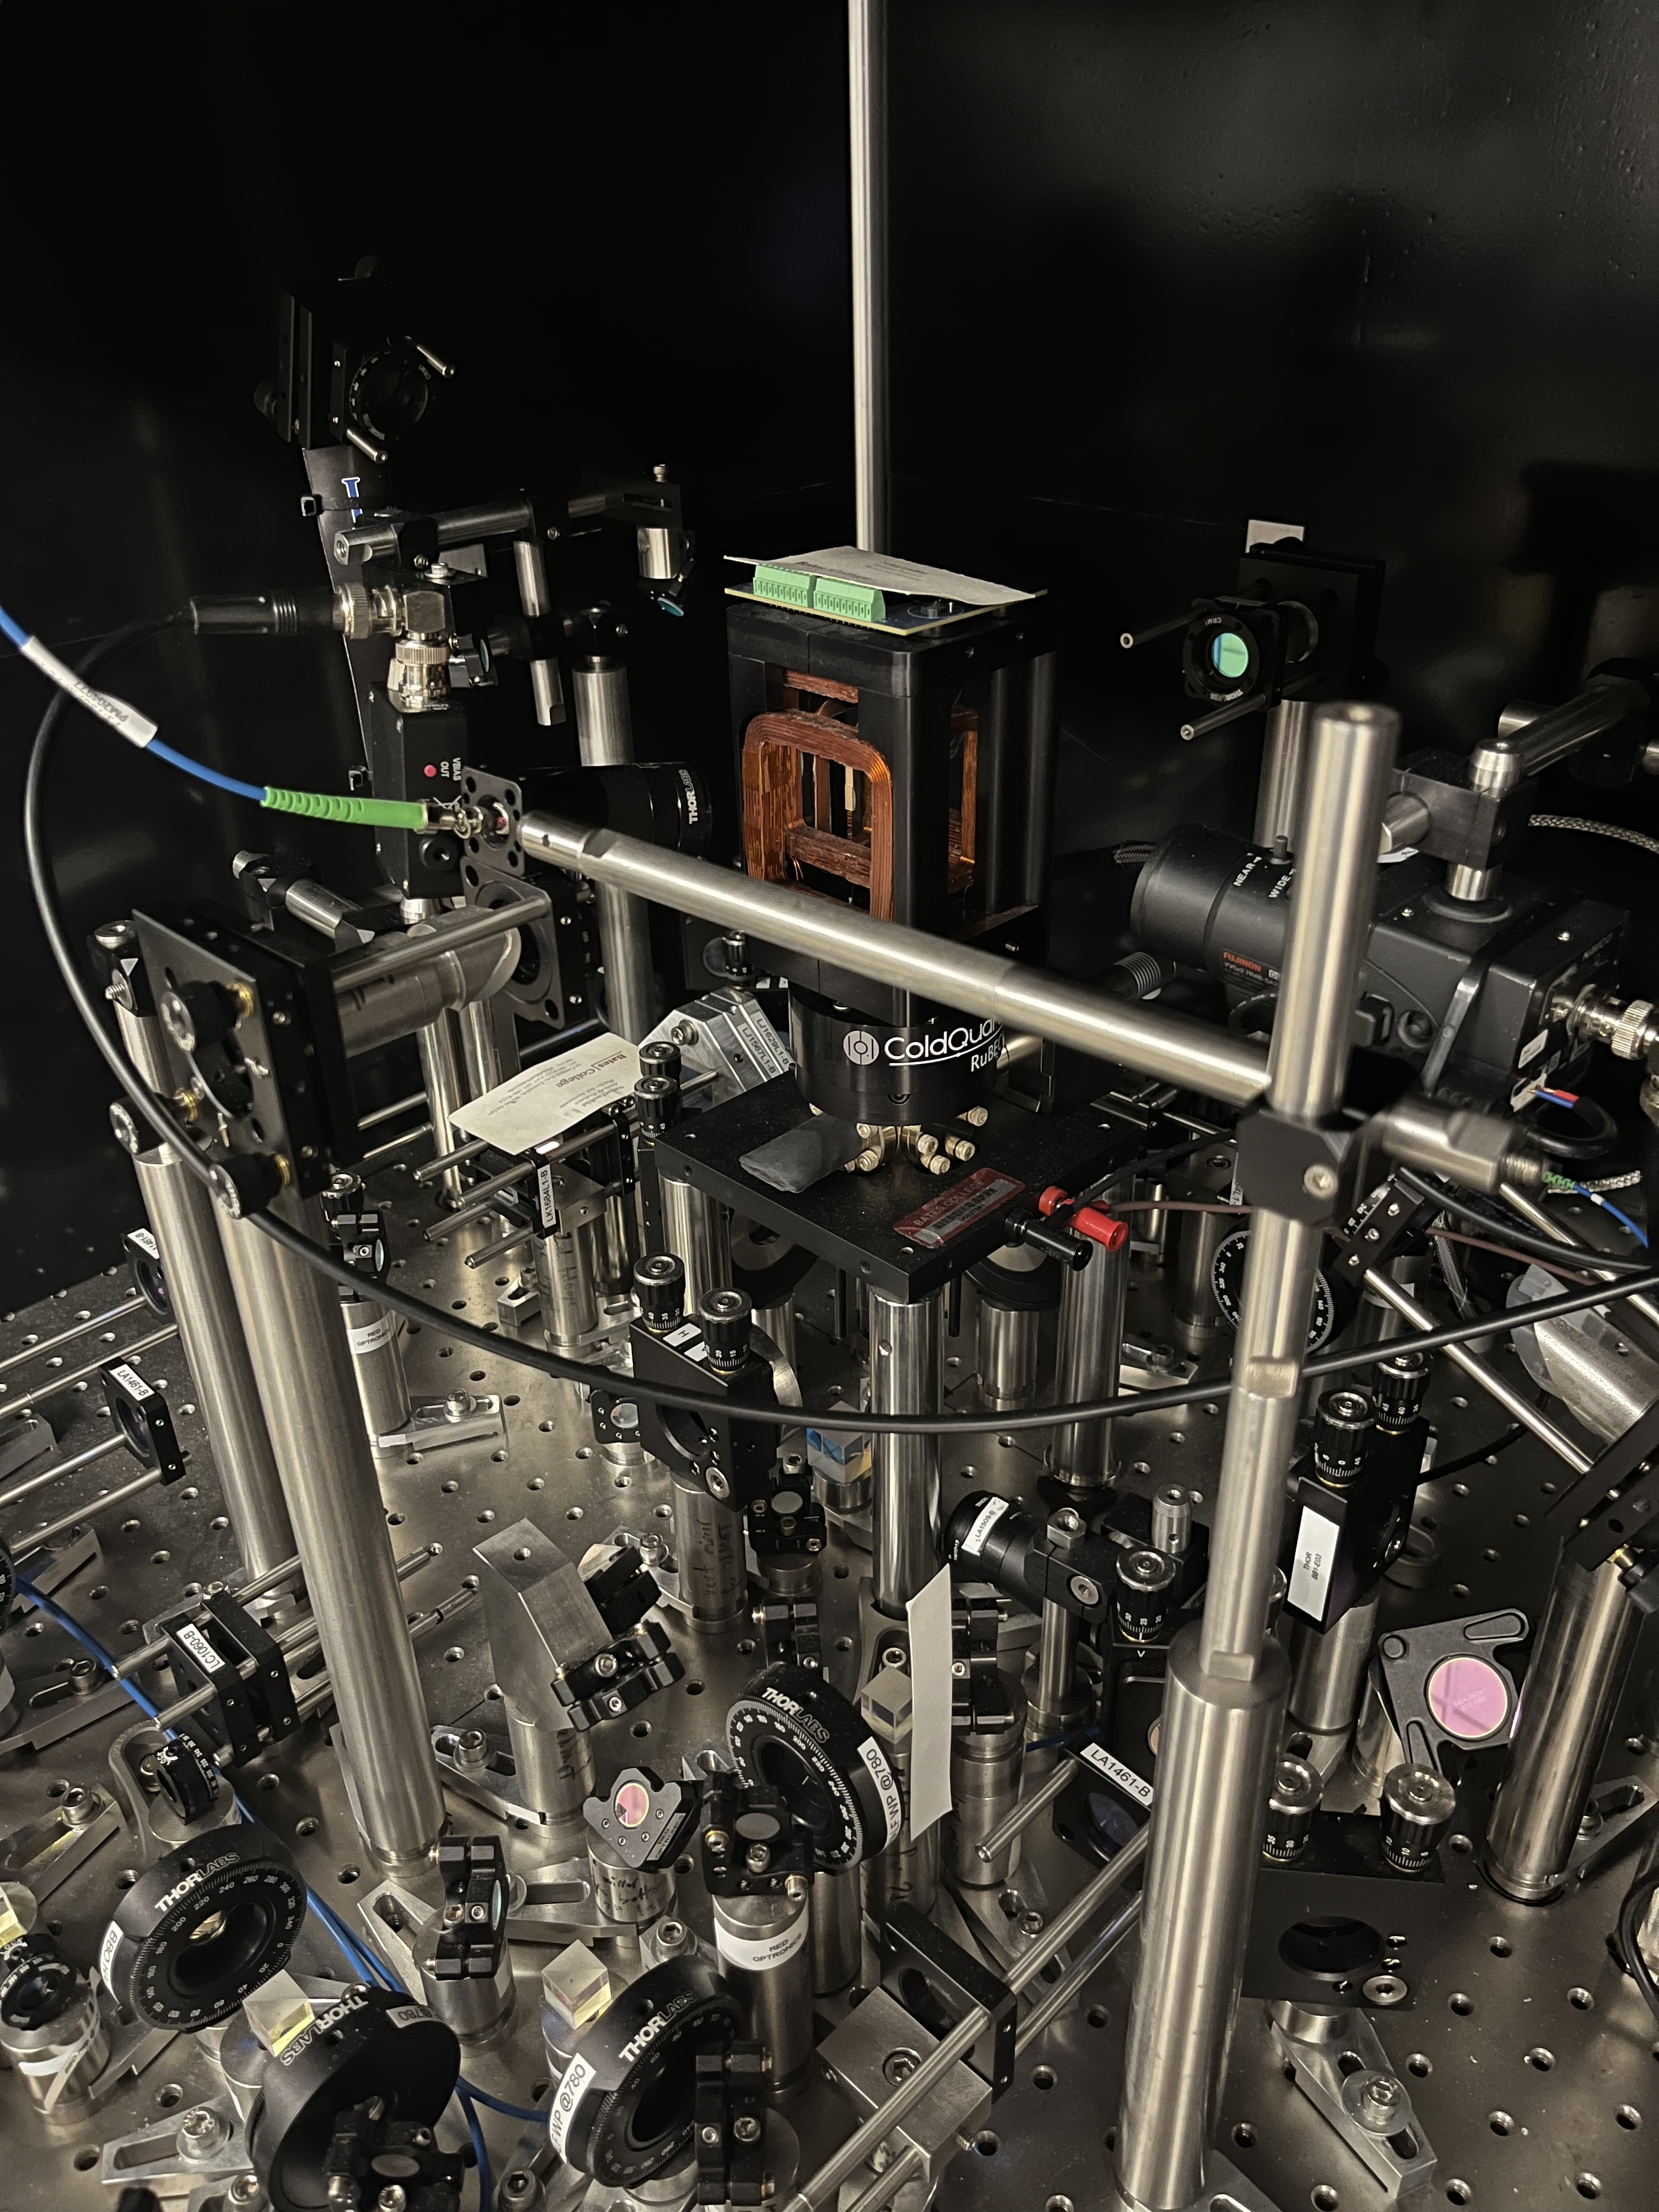
\epsfig{file=fig_shine_on_bec.jpg, scale = .11}
\end{center}
\caption{The optical pumping laser light mounted right above a principle axes. }
\end{figure}

 \section{Creating Positive Circularly Polarized Light}
 It was during this process that the optical fiber, when unscrewing it, broke. For this reason, this section will detail the steps to circularly polarizing the light, checking that it is polarized, and finalizing the optical pumping process. 

 When the light comes from out of the optical fiber it is linearly polarized. A quarter-wave plate is used to circularly polarize it. This mechanism is described in \textbf{Chapter 1.2.3}. The magnetic field from the quadrupole coil setup can then be adjusted to account for the slight misalignment from the principle axes and to make sure the atoms see positive circularly polarized light. The quarter-wave plate must be aligned in a specific way with the linear polarized light to circularly polarize the most amount of light. 
 
 To check if the the light is circularly polarized, a setup that contains a quarter-wave plate followed by a half-wave plate is used. This analyzer is shown in \textbf{Figure 3.4}. 

  \begin{figure}[h!]
\begin{center}
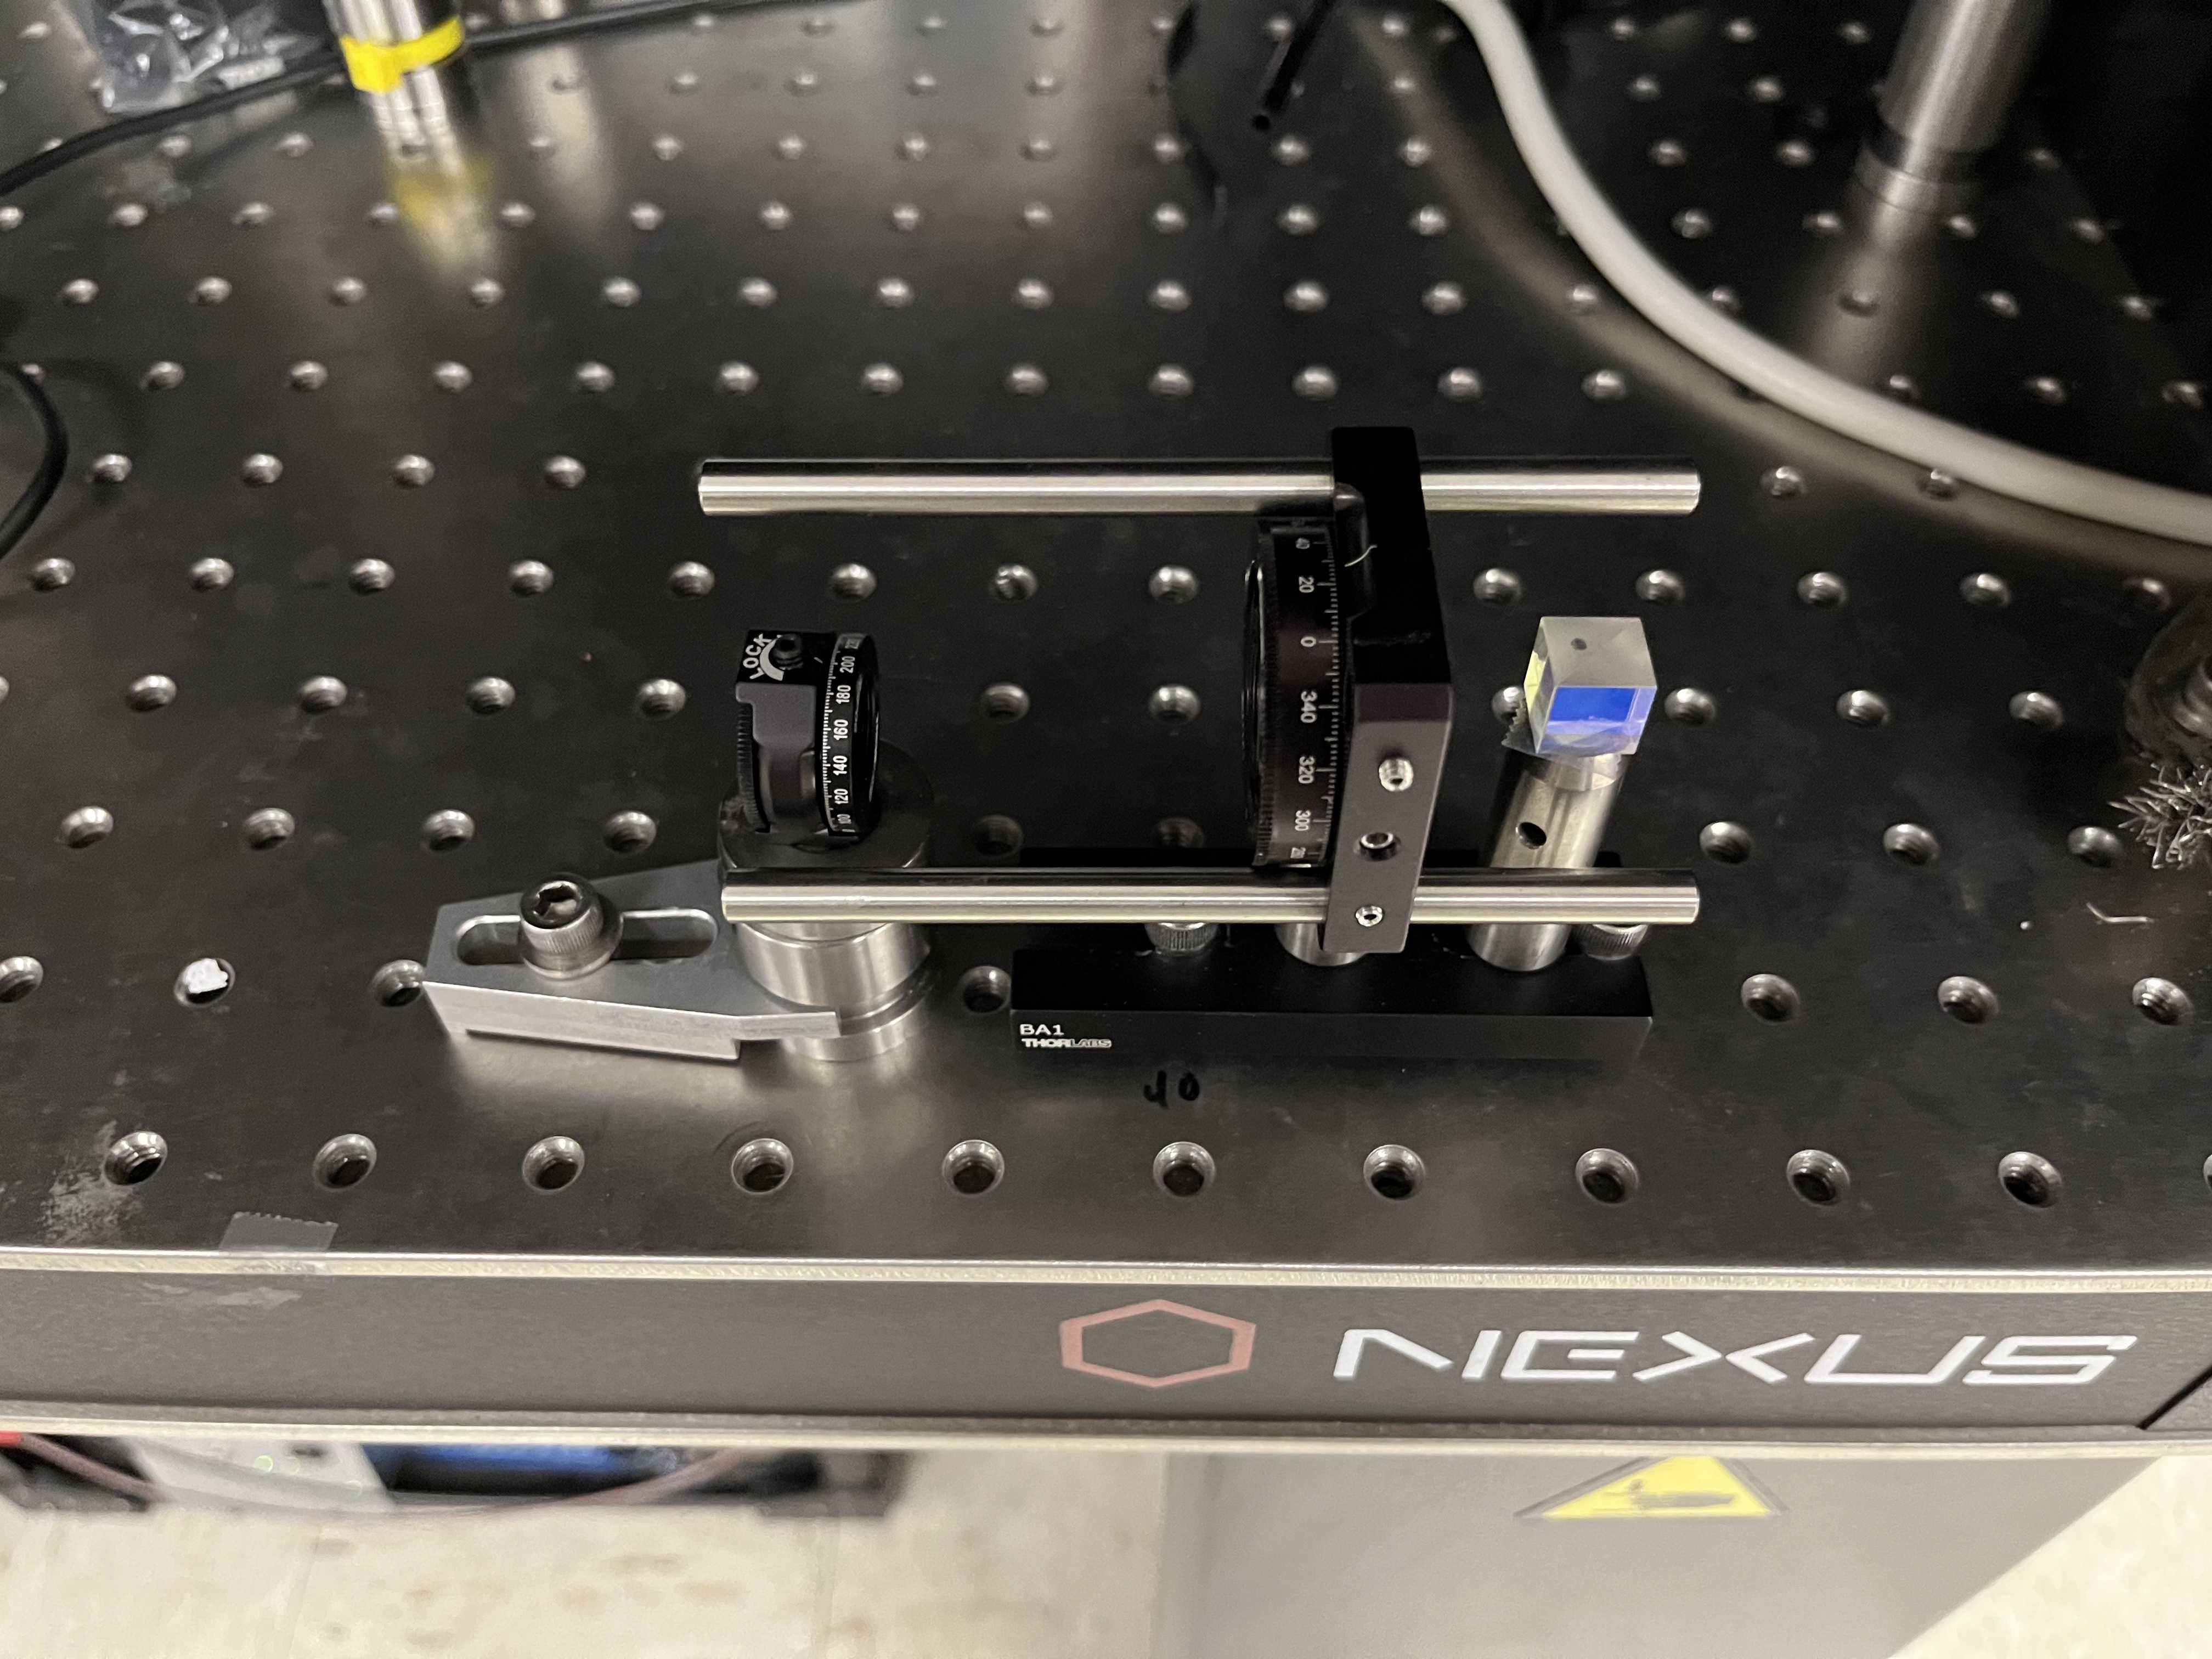
\epsfig{file=fig_polarizer_checker.jpg, scale = .11}
\end{center}
\caption{The circular polarizer analyzer. }
\end{figure}

The analyzer was clamped to the table for easy use by future students. The analyzer uses the quarter-wave plate to make the light linearly polarized. The half-wave plate is aligned so that nearly all the light will transmit through the beam splitter. If the light coming into the analyzer is not all circularly polarized, then the quarter-wave plate could circularly polarize some of it, and the half-wave plate and beam splitter will take the two orthogonal linear components of the light. This will result in a significant amount of light being reflected by the beam splitter. The student should shine the laser through this contraption and adjust the quarter-wave plate attached to the optical fiber so that as much light as possible is transmitted through the beam splitter. This is more efficiently done by minimizing the amount of light reflected by the beam splitter. These measurements are done with a power meter. 
\section{Future Steps}

A small cage mount was left for the next student. The lab should order a small cage mount that can hold the quarter-wave plate and turn to control its orientation, and of course another 10 meter optical fiber. This will make the process of mounting and checking the circular polarization easier. From there, the future steps are to create a LabVIEW process that can detune the laser and control the shutters for the optical pumping process. After that, the atoms should be caught in a magnetic trap and transferred to the chip for evaporative cooling. At that point, Bose-Einstein Condensation will be realized on the NASABEC machine. Finally, spectroscopy equipment can be used to observe the Bose-Einstein Condensate. 
